\documentclass[hyperref={hidelinks}]{beamer}
\usetheme[sectionpage=none,numbering=fraction,progressbar=frametitle]{metropolis}
\usepackage[style=ieee]{biblatex}
\usepackage{booktabs}
\usepackage{multirow}
\graphicspath{{figures/}}

\title{Aprendizagem Aplicada à Segurança}
\date{\today}

\author{Mário Antunes}
\institute{University of Aveiro}

\bibliography{references}

\begin{document}
  \maketitle

  \begin{frame}{Table of Contents}
    \tableofcontents
  \end{frame}

  \begin{frame}{Professor}
    \begin{columns}
    \column{0.7\textwidth}
      \begin{description}
        \item[Name:] Mário Antunes
        \item[E-Mail:] \href{mailto:mario.antunes@ua.pt}{\url{mario.antunes@ua.pt}}
        \item[Office:] 19.2.15 (IT1)
      \end{description}
    \column{0.3\textwidth}
      \begin{figure}
      \centering
      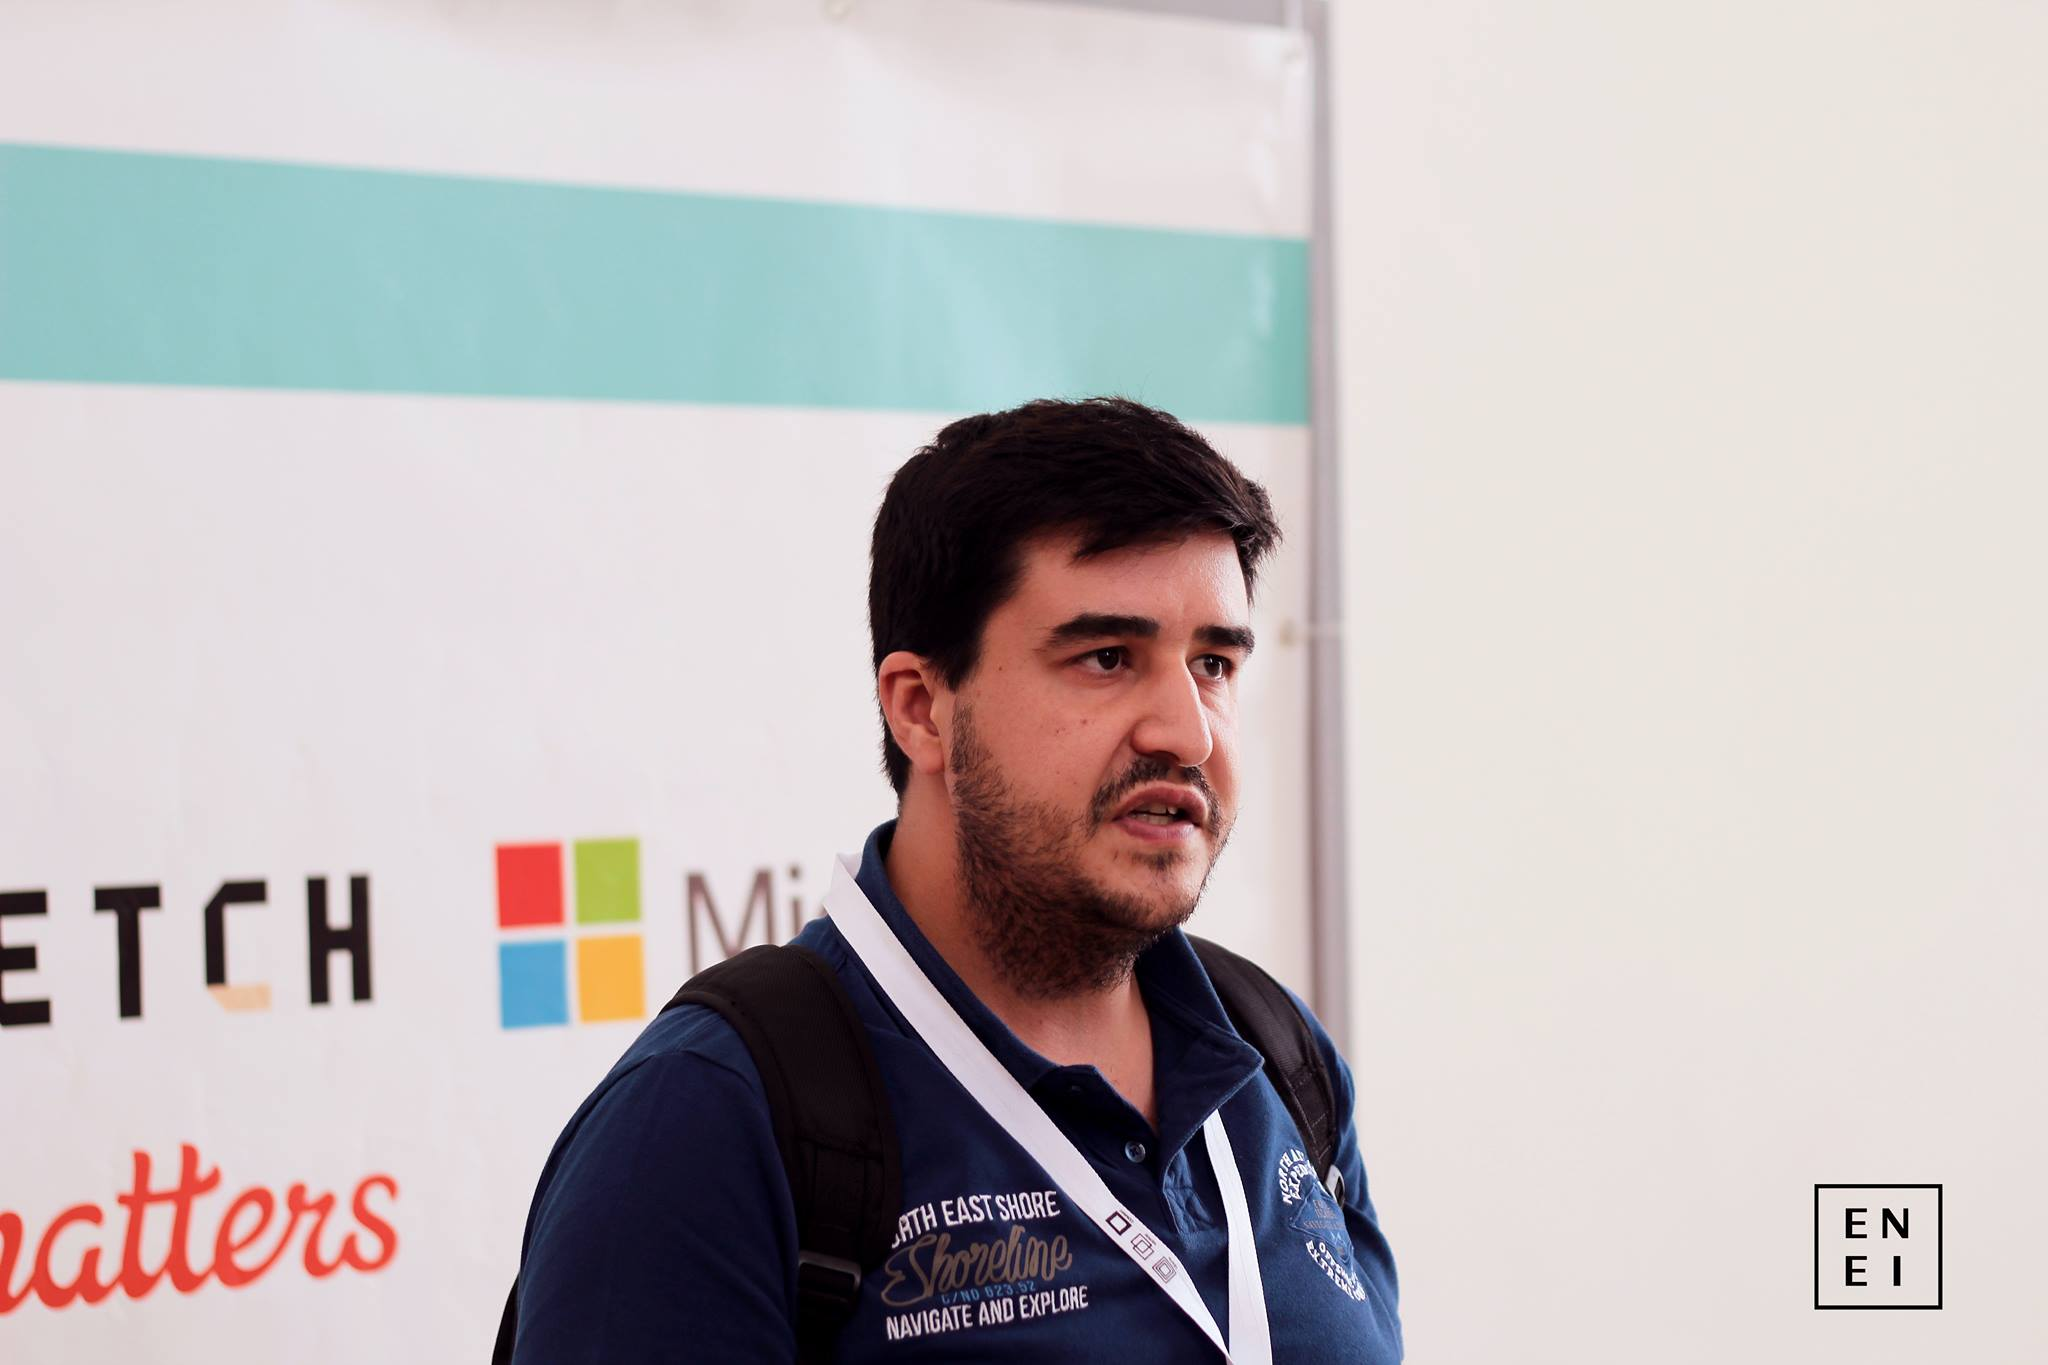
\includegraphics[width=\textwidth]{mantunes}
      \end{figure}
    \end{columns}
  \end{frame}

  \section{Class Introduction}
  \begin{frame}{Class Introduction}
    \begin{columns}
    \column{0.4\textwidth}
      \begin{itemize}
        \item Given the evolution of the threats
        \item And the complexity of the systems
        \item AI/ML are gaining traction as a usefull tool
      \end{itemize}
    \column{0.6\textwidth}
      \begin{figure}
      \centering
      
\includegraphics[width=\textwidth]{security}
      \end{figure}
    \end{columns}  
  \end{frame}

  \begin{frame}{Class Introduction}
    \begin{figure}
    \centering
    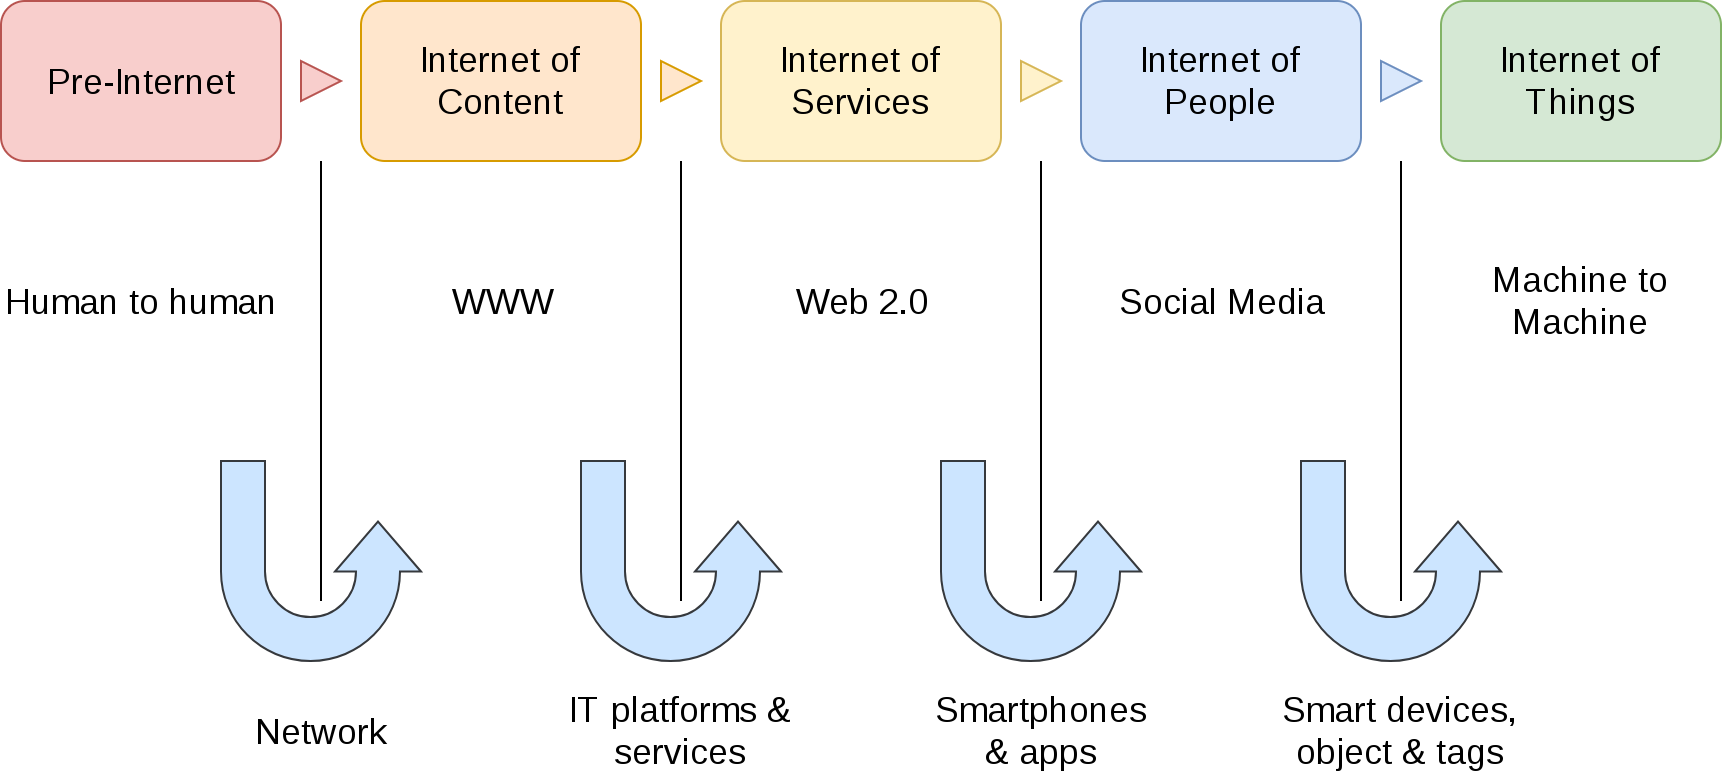
\includegraphics[width=\textwidth]{internet}
    \end{figure}
  \end{frame}

  \begin{frame}{Class Introduction}
    \begin{figure}
    \centering
    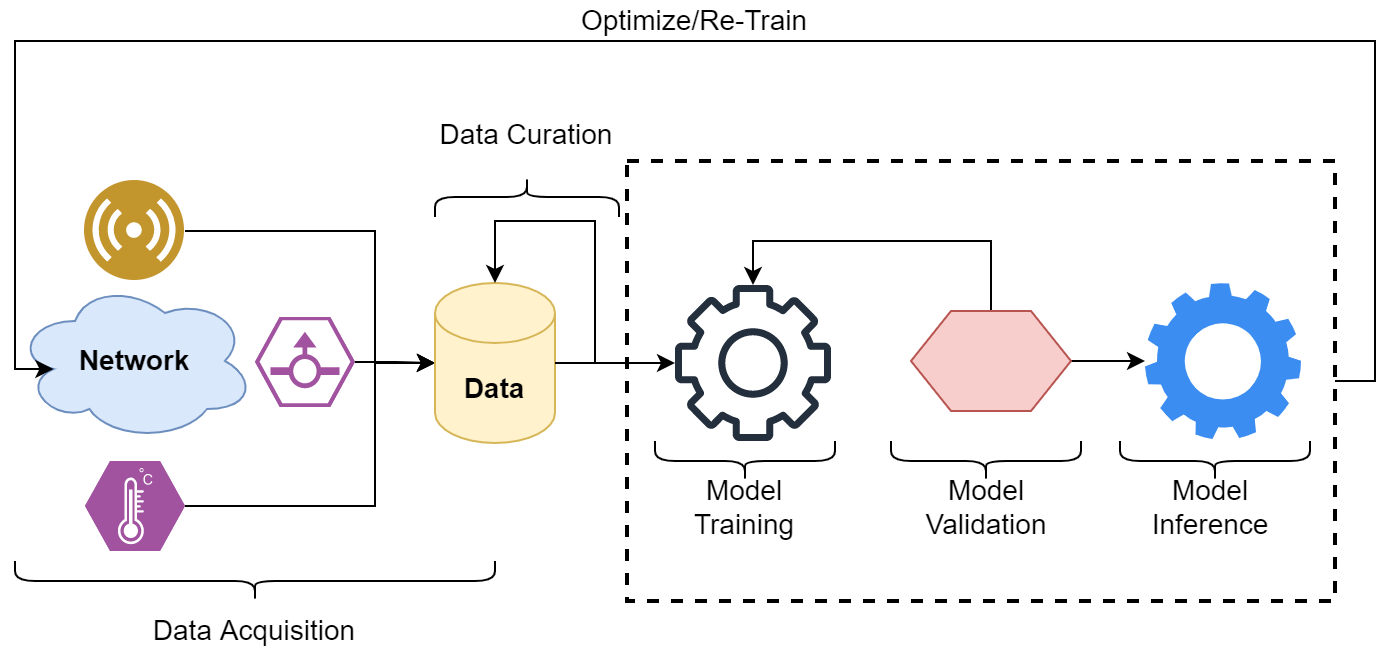
\includegraphics[width=\textwidth]{cost_learning}
    \end{figure}
  \end{frame}

  \section{Grading}
  \begin{frame}[allowframebreaks]{Grading}
    \begin{itemize}
      \item 50\% Theory + 50\% Practice 
      \item Discrete: 25\% Mid-term Exam + 25\% Final Exam + 20\% Project Idea + 30\% Project
      \item Final: 50\% Final Exame + 50\% Project 
    \end{itemize}
  \end{frame}

  \section{Class Schedule}
  \begin{frame}[allowframebreaks]{Class Schedule}
    \begin{table}[!ht]
      \footnotesize
      \centering
      \begin{tabular}{lll}
      \toprule
          Date & Class & Topic \\ \midrule
          15/09/2023 & 1 & Introduction \\ 
          22/09/2023 & 2 & \multirow{3}{*}{SPAM Detector} \\ 
          29/09/2023 & 3 \\ 
          06/10/2023 & 4 \\ 
          13/10/2023 & 5 & \multirow{3}{*}{Anomaly Detection} \\ 
          20/10/2023 & 6 \\ 
          27/10/2023 & 7 \\ 
          03/11/2023 & 8 & Mid-term Exam \\ 
          10/11/2023 & 9 & \multirow{3}{*}{Malware Analysis} \\ 
          17/11/2023 & 10 \\ 
          24/11/2023 & 11 \\ 
          01/12/2023 & 12 & \multirow{4}{*}{Project} \\ 
          08/12/2023 & 13 \\ 
          15/12/2023 & 14 \\ 
          22/12/2023 & 15 \\ \bottomrule
      \end{tabular}
  \end{table}  
  \end{frame}

  \section{Environment}
  \begin{frame}[allowframebreaks]{Environment}
    \begin{figure}
      \centering
      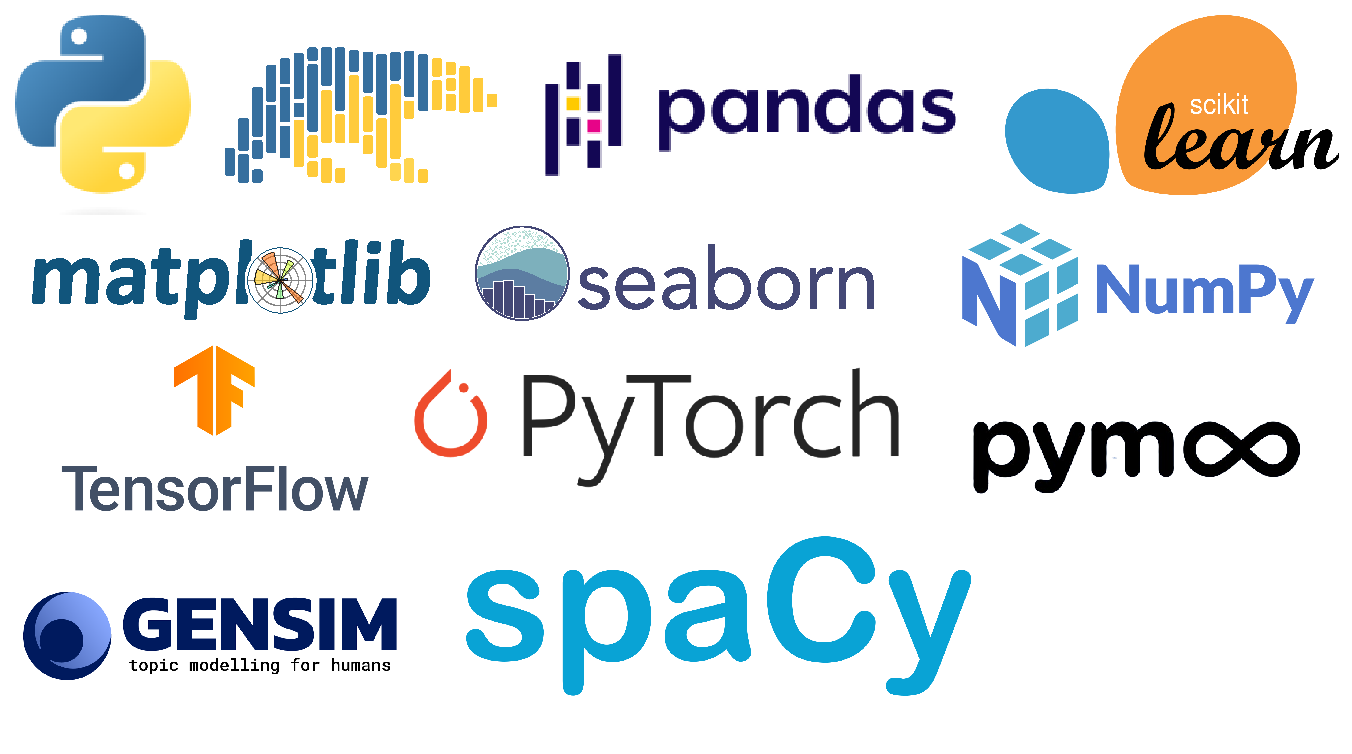
\includegraphics[width=\textwidth]{env}
      \end{figure}
  \end{frame}

  \section{Bibliography}
  \begin{frame}[allowframebreaks]{Bibliography}
    \begin{itemize}
      \item All of the books are available here:
      \href{https://learning.oreilly.com/}{\url{https://learning.oreilly.com/}}
    \end{itemize}
    \nocite{halder:2018,chio:2018,parisi:2019,tsukerman:2019,mueller:2019}
    \tiny
    \printbibliography
  \end{frame}
\end{document}